% ====================================================================
%  Self-contained source: preamble and body merged.
%  Generated by flatten.py -- edit manuscript.md and rerun
%  build.sh, not this file.
%  Compile with xelatex, twice.  Figures are expected in ../figures/;
%  for arXiv, copy them alongside and set \graphicspath{{./}}.
%  arXiv does not run BibTeX: submit main.bbl with this file.
% ====================================================================

\documentclass[11pt,a4paper]{article}
\usepackage[margin=2.4cm]{geometry}
\usepackage{amsmath,amssymb}
\usepackage{graphicx}
\usepackage{booktabs}
\usepackage{longtable}
\usepackage{array}
\usepackage{caption}
\usepackage[table]{xcolor}
\usepackage[colorlinks=true,linkcolor=black,citecolor=black,urlcolor=blue]{hyperref}
\usepackage{fontspec}
\setmainfont{DejaVu Serif}[Scale=0.92]
\setsansfont{DejaVu Sans}[Scale=0.9]
\setmonofont{DejaVu Sans Mono}[Scale=0.85]
\usepackage{unicode-math}
\setmathfont{DejaVu Math TeX Gyre}

\usepackage[numbers,sort&compress,square]{natbib}
\bibliographystyle{unsrtnat}
\usepackage{enumitem}
\setlist{nosep,leftmargin=1.4em}
\captionsetup{font=small,labelfont=bf,width=0.92\textwidth}
\graphicspath{{../figures/}}

\providecommand{\tightlist}{%
  \setlength{\itemsep}{0pt}\setlength{\parskip}{0pt}}
\providecommand{\pandocbounded}[1]{#1}

\title{\bfseries Elastic Size Misfit at Its Physical Ceiling:\\
Does Statistical Disorder Cause Solid Solution Softening in bcc Ta?\\[4pt]
\large A kink-pair kinetic Monte Carlo study of Ta(Lu)\\
with a pre-specified first-principles test}
\author{Ronghua Wu\thanks{Zhuhai Jiuchongtian Aviation Technology Co., Ltd.,
Zhuhai, China. \texttt{wrh@gdtzn.com}}
\and Ruqing Chen\thanks{GUT Geoservice Inc., Montreal, Canada.
\texttt{ruqing@hotmail.com}}}
\date{\today}

\begin{document}
\maketitle


\hypertarget{abstract}{%
\section*{Abstract}\label{sec:abstract}}

Solid solution softening in bcc metals is usually attributed to solute-induced changes in kink-pair nucleation, but the relative weight of elastic disorder and direct core chemistry has not been separated quantitatively. We address this using Ta(Lu) as an upper-bound probe. The system is not metallurgically accessible --- equilibrium solubility below 0.1 at.\% and no intermetallic phase --- but its 18.5 \% linear misfit and relaxation volume of 11.4 ų place the elastic size interaction at the ceiling attainable in a refractory host. Because the fluctuation-softening contribution scales as the square of the interaction strength while the competing hardening channels scale linearly, this system represents the most favourable case elastic disorder can present, and a negative result propagates to weaker solutes.

Combining anisotropic Stroh fields --- which we show give the \(\tfrac12\langle111\rangle\) screw a \(\cos 3\theta/r\) dilatational field that vanishes identically under the usual isotropic assumption --- with semi-grand-canonical sampling of the solute atmosphere and kink-pair kinetic Monte Carlo, we find that a random Lu field raises the flow stress of the rate-controlling ½⟨111⟩ screw at every temperature from 100 to 450 K. The fluctuation-induced barrier reduction reaches 85 meV at 100 K, 9.4 \% of the pure nucleation enthalpy, but is outweighed by kink-migration drag and by an extreme-value bias in the nucleation saddle that is partly a feature of the discretised model and which we retain as a conservative choice.

Introducing a phenomenological chemical softening reverses the sign only above κ* = 0.17 ± 0.03 eV at 150 K, 19 \% of the pure kink-pair enthalpy, and no value of κ produces softening above \textasciitilde250 K. We offer κ* as a falsifiable threshold for first-principles core calculations, noting that it is defined relative to a placeholder core binding energy and must be recomputed alongside it.

\begin{center}\rule{0.5\linewidth}{0.5pt}\end{center}

\hypertarget{introduction}{%
\section{Introduction}\label{sec:introduction}}

Adding solute to a metal normally raises its flow stress. In body-centred cubic metals below roughly 0.2 T\_m the opposite is sometimes observed: W(Re), Mo(Re) and Fe(Si) all soften on alloying before hardening at higher temperature \cite{christian1983}. The effect is technologically consequential --- it is one route to ductilising refractory metals --- and it has resisted a settled explanation for six decades.

Low-temperature plasticity in bcc metals is controlled by ½⟨111⟩ screw dislocations \cite{hirth1982,dezerald2014}, whose compact non-planar cores give them a high Peierls stress and a glide mechanism proceeding by thermally activated kink-pair nucleation. Softening must therefore act on that mechanism, and two routes are usually invoked:

\textbf{(M1) Statistical.} A random solute field makes the kink-pair nucleation barrier a random variable. Nucleation samples the low tail of its distribution, so for a Gaussian barrier distribution of variance σ² the effective activation enthalpy is reduced by \(\sigma^2/2k_BT\) \cite{labusch1970,kocks1975}. This term grows as temperature falls, so disorder alone can in principle soften a bcc metal at low temperature without any chemical effect whatsoever.

\textbf{(M2) Chemical.} The solute alters the core electronically, lowering the Peierls barrier itself. This lies outside continuum elasticity.

The two are not distinguished by observing softening; both predict it, with the same sign and a similar temperature dependence. They are distinguished by asking whether M1 is \emph{sufficient} --- and that question has a clean computational form, because M1 is entirely determined by elastic quantities that can be computed exactly.

This paper asks that question at the point where M1 is strongest. We construct a solute--dislocation model at the physical ceiling of the elastic size effect, propagate it through atomistic and mesoscale simulation, and measure whether softening appears. It does not. We then quantify what a chemical mechanism would have to supply --- a threshold \(\kappa^*\) that is strictly relative to the core binding energy assumed, and which must be recomputed alongside it --- and preregister that number as a target for first-principles calculation.

\begin{center}\rule{0.5\linewidth}{0.5pt}\end{center}

\hypertarget{why-talu}{%
\section{Why Ta(Lu)}\label{sec:why-talu}}

Ta(Lu) is not a candidate structural alloy. The equilibrium solubility of Lu in Ta lies below 0.1 at.\%, no intermetallic phase exists, and the relevant experimental setting is a supersaturated film grown far from equilibrium by molecular beam epitaxy or magnetron sputtering. We adopt it deliberately, and the choice is load-bearing rather than incidental.

With r\_Lu = 1.73 Å and r\_Ta = 1.46 Å the linear misfit is 18.5 \%, among the largest available in any refractory host. Taking the relaxation volume from measured atomic volumes,

\[\Omega_{\mathrm{Ta}} = a_0^3/2 = 18.07\ \text{\AA}^3,\qquad \Omega_{\mathrm{Lu}} = \tfrac{\sqrt{3}}{4}a^2c = 29.5\ \text{\AA}^3 \;\Longrightarrow\; \Delta V = 11.45\ \text{\AA}^3,\]

which agrees to 5\% with the hard-sphere estimate \(\Omega_{\mathrm{Ta}}[(1+\varepsilon)^3-1] = 12.0\),\AA\(^3\). Note that the linearisation \(\Delta V \simeq 3\Omega\varepsilon\), valid only for small \(\varepsilon\), would give 0.555 rather than 0.664 for \(\Delta V/\Omega\) --- a \$\sim\$20\% error that propagates as roughly 25 \% into the critical stress.

The scaling argument makes the extreme misfit essential:

\begin{itemize}
\tightlist
\item
  the M1 softening term scales as \(\sigma^2/2k_BT\), hence as \textbf{U²}, where U is the solute--dislocation interaction strength;
\item
  the competing hardening channels --- kink-migration drag, and the extreme-value bias of the nucleation saddle --- scale as \textbf{U}.
\end{itemize}

The softening-to-hardening ratio therefore grows \textbf{linearly with misfit}. Ta(Lu) is the most favourable case M1 can present in a bcc host. A negative result propagates to weaker solutes rather than being confined to this system. We state in advance that a positive result would \emph{not} have this property and would be reported as system-specific.

\begin{center}\rule{0.5\linewidth}{0.5pt}\end{center}

\begin{figure}[htbp]\centering
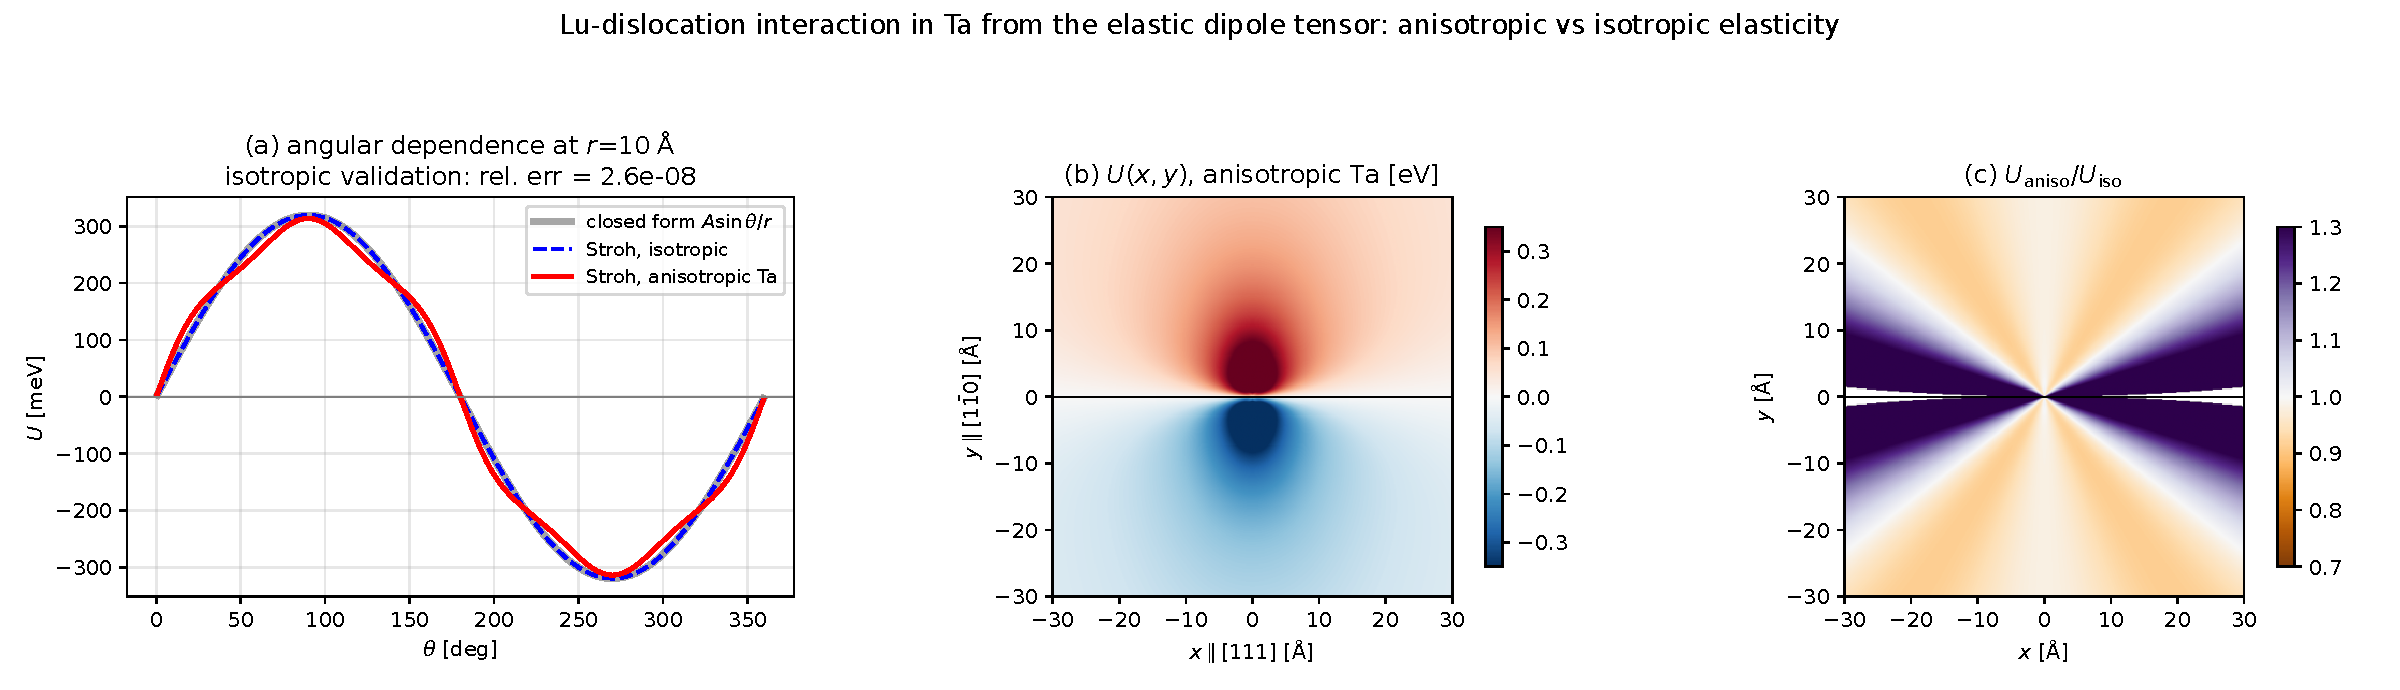
\includegraphics[width=1.0\linewidth]{fig1_elastic_fields.pdf}
\caption{Solute--dislocation interaction from the elastic dipole tensor. (a) angular dependence at $r=10$\,\AA; the isotropic Stroh solution reproduces the closed form $A\sin\theta/r$ to $2.6\times10^{-8}$. (b) anisotropic field of the edge dislocation. (c) ratio of anisotropic to isotropic: the amplitude changes by only $-1.8\%$ but the angular shape deviates by up to $\pm30\%$ near the glide plane, which is where $\mathrm{d}U/\mathrm{d}x$ controls pinning.}
\label{fig:fig1}
\end{figure}

\hypertarget{methods}{%
\section{Methods}\label{sec:methods}}

\hypertarget{elastic-fields}{%
\subsection{Elastic fields}\label{sec:elastic-fields}}

The solute--dislocation interaction is computed from the elastic dipole tensor,

\[U(r,\theta) = -P_{ij}\,\varepsilon_{ij}^{\rm disl}(r,\theta),\]

with the dislocation strain field from the anisotropic Stroh sextic formalism \cite{stroh1958,hirth1982} using the elastic dipole framework of Clouet \emph{et al.} \cite{clouet2018} and Ta elastic constants \cite{featherston1963} C₁₁/C₁₂/C₄₄ = 266.0/158.2/87.4 GPa (Zener anisotropy A = 1.622, K = 194.1 GPa).

\textbf{A symmetry result that constrains the whole treatment.} A substitutional solute on a bcc lattice site carries the full O\_h site point group. A symmetric second-rank tensor invariant under O\_h must be isotropic, so

\[\boxed{P_{ij} = P\,\delta_{ij}\ \text{exactly}},\qquad P = K\,\Omega_{\rm rel} = 13.87\ \text{eV},\]

\emph{regardless of how large the misfit is.} There is no first-order tetragonal distortion and no Fleischer shear coupling \cite{fleischer1962} for a substitutional solute in a cubic host. Shear coupling enters only at second order through the diaelastic polarisability \(\alpha_{ijkl} = -\partial P_{ij}/\partial\varepsilon_{kl}\). This is the qualitative difference from interstitial solutes such as C in bcc Fe, whose octahedral site symmetry gives a tetragonal dipole and a large first-order coupling to shear.

Consequently only the dilatation ε\_kk enters, and the interaction reduces to \(U = -P\varepsilon_{kk}\).

The implementation was validated against the closed-form isotropic result U = A sinθ/r, with \(A = (1+\nu)\mu b\Delta V/[3\pi(1-\nu)] = 3.196\) eV\(\cdot\)\AA, to a maximum relative error of \textbf{\(2.6\times10^{-8}\)}.

Core regularisation is smooth,

\[U = \frac{A\,r\sin\theta}{r^2 + r_c^2},\qquad r_c = \frac{A}{2U_{\rm cap}},\]

reducing to the far field for r ≫ r\_c, vanishing at the core, and peaking at exactly U\_cap. A hard cutoff instead places a step of ≈0.4 eV in U(x); its numerical derivative is a force spike of height ∝1/dx and width ∝dx, and we found this produced a 57 \% drift of the critical stress with grid spacing, non-monotonically (Section 5.1).

Line tensions use the de Wit--Koehler orientation dependence \cite{dewit1959} Γ = E + d²E/dθ²:

\[\Gamma_{\rm edge} = \frac{\mu b^2(1-2\nu)}{4\pi(1-\nu)}\ln\frac{R}{r_0} = 0.940\ \text{eV/\AA},\qquad \Gamma_{\rm screw} = \frac{\mu b^2(1+\nu)}{4\pi(1-\nu)}\ln\frac{R}{r_0} = 3.935\ \text{eV/\AA}.\]

For Ta, 1−2ν = 0.32: an edge dislocation is only 0.53× as stiff as the common μb²/2 estimate, while a screw is 4.19× stiffer than an edge. Since Friedel statistics \cite{friedel1964} give \(\tau \propto \Gamma^{-1/2}\), the naive estimate is wrong by 37 \% for edges.

\hypertarget{solute-atmospheres}{%
\subsection{Solute atmospheres}\label{sec:solute-atmospheres}}

The equilibrium occupancy of a lattice-gas atmosphere follows the Fermi--Dirac (McLean--Langmuir) isotherm

\[c(r,\theta) = \frac{c_0\,e^{-U/k_BT}}{1 - c_0 + c_0\,e^{-U/k_BT}},\]

which is essential here rather than cosmetic: with \(\beta|U|\) reaching 20 at the core, the Boltzmann form \(c = c_0 e^{-\beta U}\) would give c \textasciitilde{} 10⁸.

The c = ½ isosurface is a circle of diameter R\_c = A/{[}k\_BT ln((1−c₀)/c₀){]} tangent to the glide plane on the tension side --- 25.6 Å ≈ 9b at 300 K and c₀ = 1 at.\%.

Solute--solute interaction enters through the quasi-chemical interchange energy \cite{guggenheim1952} ω = 2ε\_AB − ε\_AA − ε\_BB, giving the lattice-gas Hamiltonian

\[H = \sum_i U_i c_i + J\sum_{\langle ij\rangle} c_i c_j,\qquad J = -\omega,\]

with ω \textgreater{} 0 (clustering) for the immiscible Ta--Lu pair. Two-dimensional atmospheres are equilibrated by conserved Kawasaki dynamics with Metropolis acceptance. Three-dimensional atmospheres are equilibrated by semi-grand-canonical single-site sampling: the region exchanges solute with a large reservoir, which is a grand-canonical condition, and local exchange would be diffusion-limited. The chemical potential is calibrated by bisection in a field-free box so that ⟨c⟩ = c₀ exactly at every ω, rather than taken from the mean-field expression (the two differ by 2.9 meV at ω = 0.06 eV, enough to shift the far-field concentration in a 2 at.\% solution).

\hypertarget{edge-dislocation-depinning}{%
\subsection{Edge-dislocation depinning}\label{sec:edge-dislocation-depinning}}

A flexible line x(z) in the glide plane obeys

\[H = \int\!dz\left[\tfrac12\Gamma(\partial_z x)^2 - \tau b x + \mathcal{V}(x,z)\right],\qquad \mathcal{V}(x,z) = \sum_{i\,\in\,\text{slice }z} c_i\,U(x_i - x,\,y_i).\]

The atmosphere is frozen \cite{cottrell1949}. This is not an approximation of convenience: with \(Q_{\rm diff}(\mathrm{Lu\ in\ Ta})\gtrsim3.5\) eV, \(D(600\,\mathrm{K})\sim10^{-34}\) m\(^2\)/s and a single atomic hop takes \(\sim10^{14}\) years. Below \textasciitilde0.4 T\_m no coupled diffusion/glide kinetics are required; the correct architecture is to sample the solute field once, tabulate 𝒱(x,z) on a fine grid --- which removes the \(O(N_{\rm solute})\) sum from the inner loop entirely --- and then run line dynamics alone.

The critical stress is measured drag-free: the stress is ramped quasi-statically and the line relaxed to force balance at every step, with depinning declared when no equilibrium configuration exists. The pinning criterion is the \emph{existence of an equilibrium}, not a travelled distance; a line in a random landscape legitimately advances by finite amounts and re-pins, and a distance-based criterion misreads that as depinning.

\hypertarget{kink-pair-kinetic-monte-carlo}{%
\subsection{Kink-pair kinetic Monte Carlo}\label{sec:kink-pair-kinetic-monte-carlo}}

For the screw the continuous functional

\[H[x(z)] = \int\!dz\left[\tfrac12\Gamma_{\rm screw}(\partial_z x)^2 + V_P(x) + V_{\rm sol}(x,z) - \tau b x\right]\]

is a sine-Gordon problem whose solitons are kinks, with

\[E_k = \int_0^h\!\sqrt{2\Gamma V_P(x)}\,dx = \frac{2h}{\pi}\sqrt{2\Gamma V_0},\qquad \tau_P = \frac{\pi V_0}{bh}.\]

For k\_BT ≪ E\_k the line occupies only valley minima and is described by the integer valley index n\_k. The functional reduces exactly to a solid-on-solid model,

\[\boxed{\;H = E_k\sum_k\bigl|n_k - n_{k+1}\bigr| \;+\; \sum_k W[n_k,k] \;-\; \tau b h a_z\sum_k n_k\;}\]

in which V\_P has been absorbed into E\_k and the kink migration barrier E\_km. Nucleation and migration then require no special-casing: flipping a site on a flat segment costs 2E\_k automatically, one adjacent to a kink costs zero kink energy.

Kink--kink elastic attraction \(E_{\rm int}(w) = E_{kk}/w\) with \(E_{kk} = \mu b^2h^2/[8\pi(1-\nu)a_z] = 0.61\) eV·segment is added explicitly. Without it the barrier is exactly 2E\_k at every width, there is no critical nucleus, and the computed glide velocity at 100 K is \(10^{-27}\) \AA/s.

Kinetics use the rejection-free BKL algorithm \cite{bortz1975} over three event classes per site (nucleation at the optimal width, up-migration, down-migration) with rates \(r = \nu_D\exp[-(E_{km} + \max(0,\Delta E))/k_BT]\), which satisfies detailed balance. Parameters: E\_k = 0.45 eV, E\_km = 0.02 eV, τ\_P = 0.90 GPa, \(\nu_D = 10^{13}\) s\(^{-1}\). The flow stress is defined at \(\dot\gamma = 10^{-3}\) s\(^{-1}\) with \(\rho_m = 10^{12}\) m\(^{-2}\), giving \(v_{\rm target} = 3.49\times10^4\) \AA/s, and located by bisection \textbf{in log stress} with results outside the bracket reported as undefined rather than as the bracket bound.

\hypertarget{length-scale-and-dislocation-density}{%
\subsection{Length scale and dislocation density}\label{sec:length-scale-and-dislocation-density}}

Depinning from a random landscape has no thermodynamic limit. Longer segments sample weaker regions, and we measure

\[\tau_c = 1.885 - 0.107\ln N_z\qquad(\text{rms residual }0.035\ \text{GPa})\]

over N\_z = 32--2048, with no plateau even at L = 5.9 × 10³ Å --- Gumbel-type weakest-link statistics. Critical stresses are therefore reported for a stated segment length, never as intensive material constants. Unless noted, N\_z = 128 (L = 366 Å, \(\rho = L^{-2}\approx7\times10^{14}\) m\(^{-2}\)). The same fit gives 1.4, 1.3 and 1.0 GPa at \(\rho = 10^{15}\), \(10^{14}\) and \(10^{12}\) m\(^{-2}\), a testable prediction that solution strengthening rises with dislocation density.

\begin{center}\rule{0.5\linewidth}{0.5pt}\end{center}

\hypertarget{results}{%
\section{Results}\label{sec:results}}

\hypertarget{the-edge-dislocation-behaves-classically}{%
\subsection{The edge dislocation behaves classically}\label{sec:the-edge-dislocation-behaves-classically}}

Warren--Cowley analysis \cite{warren1969} of the two-dimensional atmosphere gives a result that matters for experimental interpretation. In the saturated core, c\_Lu → 1 and

\[\alpha_1 \to \delta\bigl(e^{\omega/k_BT} - 2\bigr) \to 0 \quad\text{as}\quad \delta = 1 - c_{\rm Lu} \to 0.\]

The order parameter \textbf{vanishes} in a saturated atmosphere, because there is no chemistry left to order: the strong segregation is encoded in c(r), not in α₁. Monte Carlo confirms this, with α₁ ≈ −0.03 at c\_Lu ≈ 0.86 and a maximum of 0.48 in the transition shell at c\_Lu ≈ 0.47. The spatial signature is therefore an \textbf{annulus}, not a filled disc.

A second observation follows: sliding-window α₁ measured across the concentration gradient exceeds the homogeneous quasi-chemical prediction (0.48 vs 0.28 at the peak) because a window straddling the gradient contains Lu-rich and Ta-rich subregions and registers spurious chemical order. Since the gradient length ℓ = r²k\_BT/A falls below one lattice spacing near the core, chemical short-range order \textbf{cannot be measured reliably in the core region at all} by windowed analysis of AC-STEM or EDS data.

Three-dimensional depinning of the flexible edge line, six solute realisations at N\_z = 128:

\begin{longtable}[]{@{}lll@{}}
\toprule\noalign{}
ageing fraction θ & trough depth (eV/Å) & τ\_c (GPa) \\
\midrule\noalign{}
\endhead
\bottomrule\noalign{}
\endlastfoot
0.00 (random alloy) & −0.028 & 0.16 ± 0.09 \\
0.05 & −0.096 & 0.41 ± 0.07 \\
0.25 & −0.448 & 1.25 ± 0.10 \\
1.00 (equilibrated) & −1.896 & 5.18 ± 0.17 \\
\end{longtable}

The fully aged atmosphere exceeds the theoretical shear strength \(\mu/30 = 2.30\) GPa: \textbf{breakaway is mechanically impossible}, and yield must proceed by climb, cross-slip, or nucleation elsewhere. The crossing of μ/30 occurs at θ ≈ 0.57.

Comparison with Varvenne--Curtin theory \cite{varvenne2016} requires care. VC's default line-tension parameter α = 1/12 is 3.2× softer than the Dewit--Koehler Γ\_edge used here, and \(\tau_{y0}\propto\alpha^{-1/3}\), so the default value is not a like-for-like reference. With α matched to Γ\_edge, VC predicts 0.31 GPa against our 0.16 ± 0.09 GPa --- agreement within a factor of two given the different core treatments, but not the closer agreement a mismatched comparison would suggest.

Including solute--solute interaction raises τ\_c by 1.24×, 1.46× and 1.81× at ω = 0.02, 0.04 and 0.06 eV, and moves the μ/30 crossing from θ* = 0.57 to 0.41 at ω = 0.04 eV. The J = 0 limit reproduces the analytic Fermi--Dirac profile to 0.8σ of the binomial noise floor with a bias of +0.0002, and semi-grand-canonical and Kawasaki sampling agree on the equilibrium structure within their statistical noise.

\begin{figure}[htbp]\centering

\includegraphics[width=1.0\linewidth]{fig7_atmosphere_2d.pdf}
\caption{Two-dimensional Cottrell atmosphere from conserved Kawasaki Monte Carlo at 600\,K, $c_0=2$\,at.\%. (a) elastic field with the mean-field $c=1/2$ isoline, a circle of diameter $R_c$ tangent to the glide plane. (b) equilibrium occupancy. (c) radial profile: Monte Carlo exceeds the mean-field Fermi--Dirac profile in the transition shell because of solute--solute attraction. (d) the Warren--Cowley parameter forms an \emph{annulus}, vanishing in the saturated core.}
\label{fig:fig7}
\end{figure}

\begin{figure}[htbp]\centering

\includegraphics[width=0.6\linewidth]{fig8_warren_cowley.pdf}
\caption{Warren--Cowley $\alpha_1$ against local composition. The order parameter vanishes at both $c\to0$ and $c\to1$: a saturated atmosphere carries no chemical order because it contains no chemistry. Monte Carlo points lie above the homogeneous quasi-chemical curve because a sampling window straddling the concentration gradient registers spurious order.}
\label{fig:fig8}
\end{figure}

\begin{figure}[htbp]\centering

\includegraphics[width=1.0\linewidth]{fig2_edge_depinning.pdf}
\caption{Edge-dislocation depinning. (a) critical stress against ageing fraction at $N_z=128$; the grey band above $\mu/30$ is mechanically unattainable, so a fully aged atmosphere admits no breakaway. (b) solute--solute interaction raises $\tau_c$ by up to $1.8\times$ over the Bernoulli approximation.}
\label{fig:fig2}
\end{figure}

\hypertarget{the-rate-controlling-dislocation-does-not}{%
\subsection{The rate-controlling dislocation does not}\label{sec:the-rate-controlling-dislocation-does-not}}

For the ½⟨111⟩ screw the dilatational coupling \textbf{vanishes identically in isotropic elasticity} --- we measure \(|\varepsilon_{kk}| < 1.2\times10^{-15}\) --- and survives only because (111) is not a mirror plane of m3̄m, so the Stroh sextic does not decouple into plane strain and antiplane along a ⟨111⟩ line. The surviving field was verified to be physical rather than numerical: it scales exactly as 1/r, contains a third harmonic 80× larger than any other, and is invariant under arbitrary rotation of the in-plane basis, with a sextic residual of 10⁻¹⁵.

Its amplitude is an order of magnitude below the edge case: 65 meV versus 628 meV at r = 5 Å. The second-order modulus coupling, \(\tfrac12\alpha\,\varepsilon_{\rm shear}^2\) with \(\alpha\approx|\mu_{\rm Lu}-\mu_{\rm Ta}|\Omega = 4.7\) eV, contributes only 4.9 meV --- an order of magnitude \emph{below} the first-order anisotropic term, not above it.

Combined with a line tension 4.19× stiffer, the consequences are severe. The screw trough is 76× shallower than the edge trough (−0.020 vs −1.533 eV/Å) and the maximum lattice binding is −0.050 vs −0.411 eV, giving

\[\boxed{\;\tau_c^{\rm screw}/\tau_c^{\rm edge} < 10^{-3}\;}\] at every ageing fraction.

The Cottrell atmosphere does not pin the dislocation that controls low-temperature yield. Everything in Section 4.1 applies to edge segments, which are not the bottleneck below \textasciitilde0.4 T\_m.

\hypertarget{statistical-disorder-hardens-at-every-temperature}{%
\subsection{Statistical disorder hardens, at every temperature}\label{sec:statistical-disorder-hardens-at-every-temperature}}

Kink-pair KMC with a random 2 at.\% Lu field, U\_cap = 0.30 eV, gives a landscape standard deviation \(\sigma = 0.038\) eV per segment and hence a fluctuation softening \(\sigma^2/2k_BT\) of 169, 85, 42 and 28 meV at 50, 100, 200 and 300 K --- reaching \textbf{9.4 \%} of the pure nucleation enthalpy \(2E_k = 0.90\) eV at 100 K.

The measured flow stresses:

\begin{longtable}[]{@{}llll@{}}
\toprule\noalign{}
T (K) & τ\_pure (GPa) & τ\_alloy (GPa) & ratio \\
\midrule\noalign{}
\endhead
\bottomrule\noalign{}
\endlastfoot
100 & 0.82 & 1.01 & 1.24 \\
150 & 0.24 & 0.52 & 2.20 \\
200 & 0.012 & 0.19 & 15.6 \\
300 & \textless0.001 & 0.10 & --- \\
450 & undefined & 0.03 & --- \\
\end{longtable}

Hardening at every temperature. Two channels account for the sign. The saddle is a maximum over kink-pair widths, so disorder enters through an extreme-value statistic biased toward higher barriers; and solutes independently impede kink migration along the line, a purely hardening channel that is nearly temperature-independent. Above \textasciitilde200 K pure Ta is already athermal at the imposed strain rate, so the ratio ceases to be meaningful: any obstacle can only harden.

\begin{figure}[htbp]\centering

\includegraphics[width=1.0\linewidth]{fig5_screw_kmc.pdf}
\caption{(a) the atmosphere does not pin the rate-controlling screw: $\tau_c^{\rm screw}/\tau_c^{\rm edge}<10^{-3}$ at every ageing fraction. (b) kink-pair kinetic Monte Carlo: a random Lu field raises the flow stress at every temperature from 100 to 450\,K.}
\label{fig:fig5}
\end{figure}

\hypertarget{what-a-chemical-mechanism-would-have-to-supply}{%
\subsection{What a chemical mechanism would have to supply}\label{sec:what-a-chemical-mechanism-would-have-to-supply}}

Introducing a phenomenological chemical softening κ --- a direct reduction of the nucleation barrier when a Lu atom occupies the core region swept by the nucleus, which no elastic treatment can generate ---

\[\Delta H_{kp} = \Delta H_{kp}^{\rm pure} - \kappa\,I(\mathrm{Lu}) + \delta E_{\rm elastic},\]

reverses the sign at 150 K above

\[\boxed{\;\kappa^* = 0.17 \pm 0.03\ \text{eV} = 19\%\ \text{of the pure kink-pair enthalpy.}\;}\]

At 250 K no value of κ in the scanned range produces softening, consistent with the experimental observation that bcc solid solution softening is confined to the low-temperature Peierls-controlled regime.

\begin{center}\rule{0.5\linewidth}{0.5pt}\end{center}

\begin{figure}[htbp]\centering

\includegraphics[width=1.0\linewidth]{fig6_kappa_threshold.pdf}
\caption{(a) a phenomenological chemical softening $\kappa$ reverses the sign only above $\kappa^*=0.17$\,eV at 150\,K; at 250\,K no value suffices because pure Ta is already athermal. (b) the annealed fluctuation term $\sigma^2/2k_BT$ against the quenched extreme-value limit and against $\kappa^*$.}
\label{fig:fig6}
\end{figure}

\hypertarget{numerical-validation}{%
\section{Numerical validation}\label{sec:numerical-validation}}

Every reported number rests on parameters chosen by hand, and we tested them. Two of the four were not converged as originally set, and correcting them reversed two sensitivity conclusions.

\hypertarget{a-57-grid-artefact}{%
\subsection{A 57 \% grid artefact}\label{sec:a-57-grid-artefact}}

The original hard core cutoff --- U set to ±U\_cap inside r\_core and clipped --- puts a \textbf{step of 0.44 eV} into U(x). Its numerical derivative is a spike of height ∝1/dx and width ∝dx: on a fine grid the spike is too narrow to trap the line, on a coarse grid it is smoothed away. The measured τ\_c drifted by 57 \% between dx = 0.05 and 0.20 Å and was not monotonic (1.030, 1.619, 1.094 GPa at dx = 0.05, 0.20, 0.80 Å).

With the smooth regularisation of Section 3.1, τ\_c agrees to four significant figures from dx = 0.05 to 0.20 Å, and relaxation is 16× faster.

\textbf{This reversed a published-draft conclusion.} With the hard cutoff, \(\tau_c\) scaled as \(U_{\rm cap}^{0.20}\) and we had concluded that core binding energy was six times less important than relaxation volume, and had recommended deprioritising the expensive core DFT accordingly. With the smooth core the exponent is \(\mathbf{U_{\rm cap}^{0.91}}\), against \(\Omega_{\rm rel}^{1.26}\) --- comparable importance. The low exponent was an artefact of the step saturating the spike height.

\hypertarget{parameters-that-did-converge-and-one-that-cannot}{%
\subsection{Parameters that did converge, and one that cannot}\label{sec:parameters-that-did-converge-and-one-that-cannot}}

\begin{longtable}[]{@{}llll@{}}
\toprule\noalign{}
parameter & reference & finest & deviation \\
\midrule\noalign{}
\endhead
\bottomrule\noalign{}
\endlastfoot
dx\_grid & 1.415 & 1.415 & 0.0 \% \\
n\_τ & 1.415 & 1.406 & 0.6 \% \\
R\_keep & 1.415 & 1.419 & −0.3 \% \\
N\_z & 1.415 & 1.190 & +18.9 \% \\
\end{longtable}

N\_z does not converge and should not: this is the weakest-link statistics of Section 3.5, physics rather than numerics.

Realisation-to-realisation scatter is 9.6 \%, requiring 4 realisations for ±5 \% and 24 for ±2 \%. \textbf{All critical stresses are therefore quoted to two significant figures.}

\hypertarget{other-corrections}{%
\subsection{Other corrections}\label{sec:other-corrections}}

Three further errors were found and fixed; we record them because a reader cannot otherwise judge which numbers changed.

\begin{itemize}
\tightlist
\item
  \textbf{Branch-cut accumulation.} Writing the screw dipole displacement as ln η₁ − ln η₂ lets each branch cut contribute an independent ±2π jump; summed over \textasciitilde50 periodic images this gave displacements of 25 Å against a physical bound of \textbar b\textbar/2 = 1.43 Å. The ratio form ln(η₁/η₂) takes the principal branch of the ratio and converges quickly.
\item
  \textbf{Periodicity violation.} The textbook homogeneous tilt ∂u\_i/∂x\_j = −(b\_i/A)(d × ξ)\_j applied to the atoms left a residual of 10.2 \% of \textbar b\textbar{} that did not decrease with more images. The correct condition is u(R+C\_n) − u(R) = ΔC\_n, and the image-summed field satisfies it with a \textbf{constant} offset δ\_n (verified constant to 0.1 \% of \textbar b\textbar), so the cell vectors must be adjusted by δ\_n with no strain applied to the atoms. Measuring δ\_n numerically sidesteps every sign convention; the residual falls to 0.03 \%.
\item
  \textbf{Silent bracket saturation.} Linear bisection over a narrow stress bracket pinned pure Ta at the lower bound above 200 K and the alloy at the upper bound at 100 K, making the alloy/pure ratio meaningless while appearing well-defined.
\end{itemize}

\begin{center}\rule{0.5\linewidth}{0.5pt}\end{center}

\begin{figure}[htbp]\centering

\includegraphics[width=1.0\linewidth]{fig3_convergence.pdf}
\caption{Convergence. (a) grid, stress-ramp and cutoff parameters converge to better than 1\%. (b) line length does not and should not: weakest-link statistics give a logarithmic decay with no plateau to $N_z=2048$. (c) realisation scatter of 9.6\% sets two significant figures as the reportable precision.}
\label{fig:fig3}
\end{figure}

\begin{figure}[htbp]\centering

\includegraphics[width=1.0\linewidth]{fig4_sensitivity.pdf}
\caption{Sensitivity to the two quantities still awaiting first-principles input: $\tau_c\propto U_{\rm cap}^{0.91}$ and $\propto\Omega_{\rm rel}^{1.26}$, against the Varvenne--Curtin analytic exponent of $4/3$. An earlier draft reported an exponent of $0.20$ for $U_{\rm cap}$; that was an artefact of the discontinuous core cutoff of Sec.~5.1.}
\label{fig:fig4}
\end{figure}

\hypertarget{preregistered-test}{%
\section{Preregistered test}\label{sec:preregistered-test}}

\hypertarget{calculations}{%
\subsection{Calculations}\label{sec:calculations}}

Thirty-nine first-principles calculations, none yet run, with inputs archived unmodified.

\textbf{Set A --- elastic dipole tensor and interchange energy (12 cells).} bulk and Lu-substituted bcc supercells at 16/54/128/250 atoms, plus four Lu--Lu pair cells at neighbour shells 1--4. Fixed cell, ions only (ISIF = 2), ENCUT = 500 eV, LREAL = .FALSE., Ta\_pv + Lu\_3 PAW, k-point density constant across sizes. Yields \(P_{ij} = -V(\sigma_{\rm defect} - \sigma_{\rm bulk})\) with Pulay contributions cancelling in the difference, Ω\_rel by 1/N extrapolation, and \(\omega_n = -[E(2\mathrm{Lu}@n) + E_{\rm pure} - 2E(1\mathrm{Lu})]\).

\textbf{Set B --- screw core binding (13 cells).} 7 × 7 × 1 quadrupolar dipole cell \cite{ventelon2007}, 147 atoms, anisotropic Stroh displacement field, periodicity restored by the measured slip offset. Lu is placed at ten symmetry-inequivalent columns within 7.5 Å plus a far reference at 28.1 Å. Angular sampling is deliberate: the pairs (4.08 Å, 19.1°)/(4.09 Å, 100.9°) and (5.54 Å, 46.4°)/(5.56 Å, 73.8°) sit at equal radius and different azimuth and measure the cos 3θ amplitude directly. Defines \(U_{\rm cap}^{\rm DFT} = \max_{\rm site}|E_b|\).

\textbf{Set C --- nudged elastic band (14 images).} Two runs of seven images, using the climbing-image method \cite{henkelman2000}. \textbf{Both cores translate by the same glide vector} \(g = 2.6995\) \AA~(\(= a_0\sqrt{6}/3\), easy core to next easy core, not to the intervening hard core at \(a_0\sqrt{6}/9\)): the dipole separation and hence the elastic interaction energy are unchanged, and the net plastic strain is \((b-b)\Delta x/A = 0\), so all images share one cell and no spurious elastic work enters the barrier. Images are built by regenerating the Stroh field at intermediate core positions, not by linear interpolation of coordinates, which passes through configurations with atoms displaced off their ⟨111⟩ columns.

Extraction: \[V_0^{\rm pure}L_z = E_b^{\rm pure}/2,\qquad V_0^{\rm Lu}L_z = E_b^{\rm Lu} - E_b^{\rm pure}/2.\]

\textbf{Electronic structure choices.} Lu is 4f¹⁴ with the closed shell \textasciitilde5 eV below E\_F. A Hubbard correction acts only to shift filled states rigidly and cannot alter forces or barriers; LDA+U will not be used. The 4f contribution is instead bounded by comparing barriers with f frozen in core (Lu\_3) against an explicit-f potential. Spin--orbit coupling is first-order inactive for J = 0 Lu but significant for Ta 5d; the path is converged scalar-relativistically and SOC applied as single-point corrections at the endpoints and climbing image with ISYM = 0. SOC-corrected barriers are exploratory and do not enter the decision rule.

\hypertarget{decision-rule}{%
\subsection{Decision rule}\label{sec:decision-rule}}

With \(E_k = (2h/\pi)\sqrt{2\Gamma V_0}\),

\[\kappa_{\rm DFT} = 2\bigl(E_k^{\rm pure} - E_k^{\rm Lu}\bigr) = 2E_k^{\rm pure}\left[1 - \sqrt{V_0^{\rm Lu}/V_0^{\rm pure}}\right],\]

and \(\kappa^*(U_{\rm cap}^{\rm DFT})\) obtained by rerunning the threshold scan with U\_cap := U\_cap\^{}DFT and every other parameter frozen as in Section 3:

\begin{quote}
\textbf{If \(\kappa_{\rm DFT} < \kappa^*(U_{\rm cap}^{\rm DFT})\), we will report that the chemical softening hypothesis is falsified for Ta(Lu) within this model and parameter space. If κ\_DFT ≥ κ*(U\_cap\^{}DFT), we will report it as supported, subject to the system-specificity caveat of Section 2. Both outcomes will be reported with equal prominence.}
\end{quote}

Recomputation of κ* is mandatory. The value 0.17 eV is defined relative to the placeholder U\_cap = 0.30 eV, and the fluctuation term scales as U\_cap².

Conditions rendering the test inconclusive are declared in advance so they cannot be invoked selectively: NEB non-convergence to EDIFFG = −0.01 eV/Å within 400 steps; a U\_cap\^{}DFT for which the stress bisection saturates at 150 K; failure of either sign check in Set A (Ω\_rel ≤ 0 or ω\_eff ≤ 0); or failure of the core correction \(\Delta(r,\theta) = E_b^{\rm DFT} - U_{\rm elastic}\) to decay into the DFT noise floor by r ≈ 3b, which would indicate the 147-atom cell is too small for the elastic subtraction.

\hypertarget{what-the-rule-does-not-discriminate}{%
\subsection{What the rule does not discriminate}\label{sec:what-the-rule-does-not-discriminate}}

Falsifying the chemical hypothesis would not exclude: solute modification of the kink \emph{migration} barrier rather than the nucleation barrier; solute modification of the local line tension; non-Schmid effects and the \{112\} twinning/antitwinning asymmetry of bcc screws, absent from this model; or interstitial impurity scavenging, a mechanism proposed for W(Re) with no analogue in a solute-only model. These are out of scope, not excluded.

\begin{center}\rule{0.5\linewidth}{0.5pt}\end{center}

\begin{figure}[htbp]\centering

\includegraphics[width=0.62\linewidth]{figS1_dd_map.pdf}
\caption{Differential displacement map of the screw dipole used for the first-principles cells, verifying that two opposite cores were created and that the slipped area lies between them. Periodicity residual 0.03\% of $|\mathbf{b}|$.}
\label{fig:figs1}
\end{figure}

\hypertarget{limitations}{%
\section{Limitations}\label{sec:limitations}}

Three limitations bear directly on the sign and magnitude of the central result.

\textbf{Extreme-value bias.} The solid-on-solid kinetics take the kink-pair barrier as a maximum over nucleus widths. Disorder therefore enters through an extreme-value statistic biased toward higher barriers, and this bias is a property of the discretised model rather than of the physics. It systematically favours hardening, and a formulation sampling the full saddle manifold --- a string method over the continuous functional, for instance --- would reduce the reported hardening by an amount we have not quantified. Our result is consequently a \textbf{conservative bound on softening}, not a symmetric estimate.

\textbf{Placeholder core energy.} U\_cap = 0.30 eV is taken from the range reported for oversized substitutionals at bcc screw cores in other hosts, pending Set B. The fluctuation term scales as U\_cap², so a twofold error quadruples it. κ* = 0.17 eV is a relative quantity built on this placeholder and should not be quoted independently of it.

\textbf{Literature parameters.} \(E_k = 0.45\) eV and \(\tau_P = 0.90\) GPa are literature estimates for pure Ta, not values derived for this system. \(\tau_P\) carries a known discrepancy: density-functional values near 1 GPa exceed experimental extrapolations of roughly 0.4 GPa, a disagreement common to bcc transition metals and unresolved here. Separately, \(\Omega_{\rm rel} = 11.4\) \AA\(^3\) is a hard-sphere estimate pending Set A, and \(\tau_c \propto \Omega_{\rm rel}^{1.26}\).

\textbf{Lattice topology.} This is an independent approximation, not a consequence of the parameter choices above. The solid-on-solid model maps the solute field onto a simple-cubic neighbour network (\(z=6\)) rather than the bcc first-neighbour shell (\(z=8\)). The effective interchange energy is rescaled accordingly, but the coordination change also alters the connectivity of the kink landscape in a way we have not quantified. Repeating the kinetics on the true bcc shell would test whether any part of the reported hardening depends on the lattice topology rather than on the disorder itself.

\begin{center}\rule{0.5\linewidth}{0.5pt}\end{center}

\hypertarget{conclusion}{%
\section{Conclusion}\label{sec:conclusion}}

By constructing a solute--dislocation model at the physical ceiling of the size-misfit effect, we find that elastic disorder alone does not produce solid solution softening in a bcc metal, even where its statistical advantage over the competing hardening channels is greatest. The result places the origin of softening outside continuum elasticity and inside the dislocation core, and converts a qualitative expectation into a quantitative threshold: a solute must lower the kink-pair nucleation enthalpy by ≳0.17 eV at 150 K, roughly one fifth of its pure-metal value, before the alloy yields more easily than the host.

Along the way the calculation produced three results of independent interest: a substitutional solute in a cubic host has a strictly isotropic elastic dipole regardless of misfit, so the classical Fleischer shear coupling is unavailable to it; the ⟨111⟩ screw acquires a dilatational field only through the failure of (111) to be a mirror plane, an order of magnitude weaker than the edge and insufficient to bind an atmosphere; and the Warren--Cowley order parameter vanishes inside a saturated Cottrell atmosphere, so segregation and chemical order must be measured separately rather than conflated. The last of these carries a direct instruction for experiment: anyone characterising local chemical order near a dislocation by AC-STEM or EDS must first subtract the background concentration gradient produced by elastic segregation, since a sampling window straddling that gradient registers order that is not chemical in origin --- and near the core, where the gradient length falls below one lattice spacing, no windowed measurement can separate the two at all.

Ta(Lu) is not a candidate structural alloy. As an extreme probe it bounds what elasticity can and cannot explain, and it defines a target that first-principles core calculations can meet or refute.

\begin{center}\rule{0.5\linewidth}{0.5pt}\end{center}

\hypertarget{data-availability}{%
\section*{Data availability}\label{sec:data-availability}}

All generation and analysis scripts, the CSV data layer underlying every figure, the convergence study, and every unmodified DFT input deck are available at \url{https://github.com/Ruqing1963/talu-size-misfit-softening} and archived at {[}Zenodo DOI to be assigned{]}. Output templates are archived containing zeros; the included \texttt{verify\_no\_results.sh} confirms this independently. Both extraction pipelines have been validated by synthetic round-trip tests, in which injected values of Ω\_rel and ω\_eff are recovered exactly.

\hypertarget{tool-disclosure}{%
\section*{Tool disclosure}\label{sec:tool-disclosure}}

A large language model (Anthropic Claude) was used for derivation checking, code development and manuscript drafting. Consistent with Zenodo and ICMJE guidance it is not an author: it cannot take responsibility for the work or consent to publication. All physical claims, parameter choices and the decision rule are the responsibility of the authors, who have verified the derivations independently.

\begin{center}\rule{0.5\linewidth}{0.5pt}\end{center}

\bibliographystyle{unsrtnat}
\bibliography{references}
\end{document}
